\documentclass[
11pt, % The default document font size, options: 10pt, 11pt, 12pt
codirector, % Uncomment to add a codirector to the title page
]{charter} 


% El títulos de la memoria, se usa en la carátula y se puede usar el cualquier lugar del documento con el comando \ttitle
\titulo{Aplicación web para el control de acceso en alquileres temporales mediante la gestión de periféricos} 
% Nombre del posgrado, se usa en la carátula y se puede usar el cualquier lugar del documento con el comando \degreename
\posgrado{Carrera de Especialización en Sistemas Embebidos} 
%\posgrado{Carrera de Especialización en Internet de las Cosas} 
%\posgrado{Carrera de Especialización en Inteligencia Artificial}
%\posgrado{Maestría en Sistemas Embebidos} 
%\posgrado{Maestría en Internet de las cosas}
% IMPORTANTE: no omitir titulaciones ni tildación en los nombres, también se recomienda escribir los nombres completos (tal cual los tienen en su documento)
% Tu nombre, se puede usar el cualquier lugar del documento con el comando \authorname
\autor{Ing. Andrea García}

% El nombre del director y co-director, se puede usar el cualquier lugar del documento con el comando \supname y \cosupname y \pertesupname y \pertecosupname
\director{Ing. Sergio Starkloff, CTO}
\pertenenciaDirector{SURiX} 
\codirector{} % para que aparezca en la portada se debe descomentar la opción codirector en los parámetros de documentclass
\pertenenciaCoDirector{FIUBA}

% Nombre del cliente, quien va a aprobar los resultados del proyecto, se puede usar con el comando \clientename y \empclientename
\cliente{Ing. Sergio Starkloff, CTO}
\empresaCliente{SURiX}
 
\fechaINICIO{27 de febrero de 2024}		%Fecha de inicio de la cursada de GdP \fechaInicioName
\fechaFINALPlan{16 de abril de 2024} 	%Fecha de final de cursada de GdP
\fechaFINALTrabajo{xx de mayo de 2024}	%Fecha de defensa pública del trabajo final

\usepackage{rotating}

\begin{document}

\maketitle
\thispagestyle{empty}
\pagebreak


\thispagestyle{empty}
{\setlength{\parskip}{0pt}
\tableofcontents{}
}
\pagebreak


\section*{Registros de cambios}
\label{sec:registro}


\begin{table}[ht]
\label{tab:registro}
\centering
\begin{tabularx}{\linewidth}{@{}|c|X|c|@{}}
\hline
\rowcolor[HTML]{C0C0C0} 
Revisión & \multicolumn{1}{c|}{\cellcolor[HTML]{C0C0C0}Detalles de los cambios realizados} & Fecha      \\ \hline
0      & Creación del documento                                 &\fechaInicioName \\ \hline
1      & Se completa hasta el punto 5 inclusive                & 12 de marzo de 2024 \\ \hline
2      & Se completa hasta el punto 9 inclusive                & 19 de marzo de 2024 \\ \hline
3      & Se completa hasta el punto 12 inclusive                & 26 de marzo de 2024 \\ \hline
4      & Se completa el plan	                                 & {02} de {abril} de 2024 \\ \hline

% Si hay más correcciones pasada la versión 4 también se deben especificar acá

\end{tabularx}
\end{table}

\pagebreak



\section*{Acta de constitución del proyecto}
\label{sec:acta}

\begin{flushright}
Buenos Aires, \fechaInicioName
\end{flushright}

\vspace{2cm}

Por medio de la presente se acuerda con la \authorname\hspace{1px} que su Trabajo Final de la \degreename\hspace{1px} se titulará ``\ttitle'' y consistirá en desarrollar una aplicación web en colaboración con SURiX para facilitar el ingreso a propiedades rentadas por periodos cortos mediante la interacción con dispositivos móviles de los inquilinos. El trabajo tendrá un presupuesto preliminar estimado de 580 horas y un costo estimado de \$ 4430060,73, con fecha de inicio el \fechaInicioName\hspace{1px} y fecha de presentación pública el \fechaFinalName.

Se adjunta a esta acta la planificación inicial.

\vfill

% Esta parte se construye sola con la información que hayan cargado en el preámbulo del documento y no debe modificarla
\begin{table}[ht]
\centering
\begin{tabular}{ccc}
\begin{tabular}[c]{@{}c@{}}Dr. Ing. Ariel Lutenberg \\ Director posgrado FIUBA\end{tabular} & \hspace{2cm} & \begin{tabular}[c]{@{}c@{}}\clientename \\ \empclientename \end{tabular} \vspace{2.5cm} \\ 
\multicolumn{3}{c}{\begin{tabular}[c]{@{}c@{}} \supname \\ Director del Trabajo Final\end{tabular}} \vspace{2.5cm} \\
\end{tabular}
\end{table}




\section{1. Descripción técnica-conceptual del proyecto a realizar}
\label{sec:descripcion}

El proyecto actual forma parte del programa de vinculación de la Universidad de Buenos Aires en colaboración con SURiX, una empresa líder con más de dos décadas de experiencia en soluciones IP para seguridad y control de acceso. La motivación para abordar la interacción de periféricos desde la web surge como respuesta a la ineficiencia detectada en la coordinación de la entrega de llaves, una problemática evidente en el ámbito de la renta de alojamientos colaborativos como Airbnb.

La solución propuesta se basa en una aplicación que utiliza tecnología web para ofrecer una experiencia eficiente, segura y cómoda, permitiendo el acceso a través de los periféricos de los dispositivos móviles de los usuarios. El proceso se divide en cuatro fases: integración con las APIs de Bluetooth y grabación de audio, diseño y desarrollo de la página web, pruebas y ajustes, y finalmente, la implementación y lanzamiento del sistema.

En el ámbito comercial, las cerraduras digitales son comúnmente utilizadas para transformar la seguridad residencial en este ámbito. Sin embargo, la presente iniciativa está basada en la web y se destaca por su enfoque en la accesibilidad e interoperabilidad, a diferencia de los dispositivos que a menudo requieren aplicaciones propias. El contar con un aplicativo privado constituye una restricción, ya que suele depender de las actualizaciones del sistema operativo, además la creciente variedad de dispositivos puede generar desafíos en términos de compatibilidad y desarrollo.

La lógica de funcionamiento del proyecto en mención utiliza recursos web para interactuar con la cámara, Bluetooth y audio del teléfono móvil del inquilino. Esto permite acciones como el escaneo de códigos QR, validación de información, apertura de puertas, comunicación a través de bluetooth y un buzón de voz para mensajes entre inquilino y propietario tal como se muestra en la figura \ref{fig:diagBloques}. La facilidad de uso, interfaz intuitiva y accesibilidad universal resaltan la singularidad del proyecto, respaldado por la experiencia de SURiX en soluciones tecnológicas innovadoras.

\begin{figure}[htpb]
\centering 
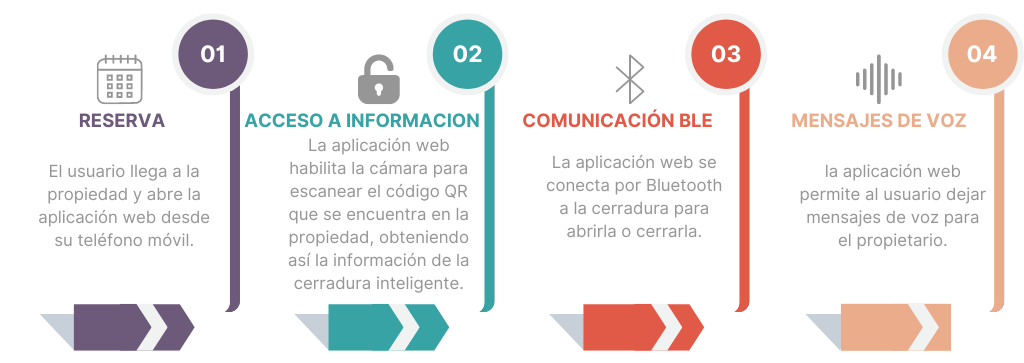
\includegraphics[width=1\textwidth]{./Figuras/flowchart.png}
\caption{Diagrama en bloques del sistema.}
\label{fig:diagBloques}
\end{figure}

Este prototipo, si bien integra la aplicación web con periféricos del teléfono, no involucra bases de datos para inquilinos o propietarios y carece de controles temporales para el acceso. Asimismo, prescinde de un sistema de inicio de sesión y, en relación al buzón de voz, propone un modelo donde los mensajes del usuario se convierten en mensajes recibidos lo que establece un ciclo continuo. Este diseño simplificado concuerda con el propósito demostrativo del proyecto, enfocándose en la esencial interacción web-periférico.  

\section{2. Identificación y análisis de los interesados}
\label{sec:interesados}

Para llevar a cabo este proyecto de colaboración entre la empresa asociada y la UBA, se requiere la participación de varios individuos. A continuación en el cuadro \ref{tab:interesados}, se detalla a los involucrados:
\begin{table}[ht]
\caption{Identificación de los interesados}
\label{tab:interesados}
\begin{tabularx}{\linewidth}{@{}|l|X|X|l|@{}}
\hline
\rowcolor[HTML]{C0C0C0} 
Rol           & Nombre y Apellido & Organización 	& Puesto 	\\ \hline
%Auspiciante   &        -          &        -        &         -          \\ \hline
Cliente       & SURiX      &\empclientename	& Empresa de vinculación\\ \hline
%Impulsor      &        -          &        -        &        	\\ \hline
Responsable   & \authorname       & FIUBA        	& Alumno 	\\ \hline
%Colaboradores &        -          &        -        &        -          \\ \hline
Orientador    & \clientename      &\empclientename	& Director del Trabajo Final\\ \hline
Equipo        & Leslie Queglas \newline 
			Estefanía Del Valle Fiorabanti & SURiX &Full Stack Developers\\ \hline
%Opositores    &        -          &         -       &        -          \\ \hline
%Usuario final &        -          &         -       &        -          \\ \hline
\end{tabularx}
\end{table}

\begin{itemize}
        \item Cliente: SURIX, fundada en 1998, es una empresa que ofrece soluciones de comunicación y control de acceso IP y analógico.
        \item Responsable: Andrea García, es la persona encargada del desarrollo del aplicativo web y la realización de pruebas.
	\item Orientador: Sergio Starkloff, fundador de SURiX, lidera la propuesta en calidad de director del trabajo final. Define los requisitos tecnológicos clave para resolver la problemática central del proyecto.
	\item Equipo: los miembros del equipo, Leslie Quetglas y Estefanıa Del Valle Fiorabanti, forman parte de SURiX como desarrolladoras Full Stack y apoyan a la responsable en temas de Front End del presente proyecto.
	
\end{itemize}

\section{3. Propósito del proyecto}
\label{sec:proposito}

El propósito de este proyecto es abordar la ineficiencia en la coordinación de la entrega de llaves en el alquiler de alojamientos temporarios, mediante el desarrollo de una aplicación web innovadora que permita el acceso a través de los dispositivos móviles de los usuarios, interactuando con los periféricos correspondientes. Se busca mejorar la experiencia de los usuarios y optimizar la gestión de las propiedades, ofreciendo una solución integral basada en la accesibilidad, interoperabilidad y seguridad proporcionadas por la tecnología web.
\newpage
\section{4. Alcance del proyecto}
\label{sec:alcance}

El proyecto incluye:
\begin{itemize}
	\item Desarrollo de una aplicación web para la gestión de acceso a alojamientos temporarios.
        \begin{itemize}
    		\item Integración con APIs de Bluetooth y grabación de audio.
    		\item Diseño y desarrollo de la interfaz de usuario.
        \end{itemize}
	\item Pruebas y ajustes del sistema.
\end{itemize}

El proyecto no incluye:
\begin{itemize}
	\item Implementación de una base de datos para gestionar información de inquilinos o propietarios.
        \item Control de fechas y horarios para el acceso.
        \item Sistema de inicio de sesión.
	\item Desarrollo de hardware para dispositivos de acceso.
\end{itemize}

\section{5. Supuestos del proyecto}
\label{sec:supuestos}
Para el desarrollo del presente proyecto se supone que:

\begin{itemize}
	\item Se dispone del equipo necesario para llevar a cabo pruebas de comunicación entre periféricos y hardware, lo cual incluye dispositivos móviles compatibles con Bluetooth y acceso a servidores propios proporcionados por SURiX para alojar la aplicación web.
	\item Existe acceso a herramientas de desarrollo de software y entornos de prueba para garantizar la funcionalidad y compatibilidad del sistema en diferentes dispositivos móviles.
	\item Se cuenta con un ambiente de pruebas adecuado para simular escenarios de uso real y verificar la interoperabilidad de los periféricos con la aplicación web.
        \item El personal técnico tiene el conocimiento y la capacitación necesarios para llevar a cabo las pruebas de manera efectiva y resolver cualquier problema que pueda surgir durante el proceso de desarrollo.
\end{itemize}

\section{6. Requerimientos}

\subsection{Requerimientos funcionales}
\begin{enumerate}
\item Los usuarios deben poder visualizar la información de la propiedad correspondiente para alquiler temporal (prioridad menor).
\item Los usuarios deben poder utilizar los periféricos de su teléfono móvil para interactuar con la aplicación (prioridad mayor).
\item La aplicación web debe proporcionar una funcionalidad de escaneo de códigos QR para acceder a la información de la propiedad (prioridad mayor).
\item Una vez escaneado el código QR, la aplicación debe proporcionar al usuario la información necesaria para conectarse por Bluetooth con la cerradura electrónica de la propiedad (prioridad mayor).
\item La aplicación debe permitir al usuario abrir o cerrar la cerradura electrónica utilizando la funcionalidad de activación Bluetooth (prioridad mayor).
\item El sistema debe notificar al propietario cuando la cerradura electrónica se abre o se cierra (prioridad menor).
\item La aplicación web debe facilitar la comunicación entre el inquilino y el propietario mediante mensajes de voz (prioridad mayor).
\item La aplicación debe ser compatible con el navegador web Chrome con versión mínima 85 en sistema operativo Android (prioridad mayor).
\item Todos los mensajes de voz y la información relacionada deben estar alojados en los servidores de SURiX (prioridad menor).
\end{enumerate}

\subsection{Requerimientos de documentación}
\begin{enumerate}
\item Se debe incluir un manual de usuario que explique cómo utilizar todas las funciones de la aplicación (prioridad mayor).
\item La documentación técnica debe describir la arquitectura del sistema y los requisitos de hardware y software necesarios para su implementación (prioridad menor).
\end{enumerate}

\subsection{Requerimientos de testing}
\begin{enumerate}
\item Se deben realizar pruebas exhaustivas de funcionalidad para asegurar que todas las características de la aplicación funcionen correctamente (prioridad mayor).
\item Se deben llevar a cabo pruebas de compatibilidad para verificar que la aplicación sea compatible con determinados dispositivos móviles y navegadores web (prioridad mayor).
\item Se deben realizar pruebas de seguridad para identificar posibles vulnerabilidades y asegurar la protección de los datos de los usuarios (prioridad menor).
\end{enumerate}

\subsection{Requerimientos de interfaz}
\begin{enumerate}
\item La interfaz de usuario debe ser intuitiva y fácil de navegar (prioridad mayor).
\item Se debe proporcionar retroalimentación visual para confirmar las acciones realizadas por el usuario, como el acceso a la propiedad o el envío de un mensaje de voz (prioridad menor).
\item La aplicación debe contar con un diseño \textit{responsive} que se adapte automáticamente a diferentes tamaños de pantalla (prioridad menor).
\end{enumerate}

\section{7. Historias de usuarios (\textit{Product backlog})}
\label{sec:backlog}

\subsection{Roles}
\begin{itemize}
\item Inquilino: usuario que alquila una propiedad temporalmente y necesita acceder a través de la aplicación web.
\item Propietario: usuario que ofrece propiedades en alquiler temporal y necesita gestionar el acceso de los inquilinos.
\end{itemize}

\subsection{Puntos de historia}
Para la ponderación de cada historia de usuario, se hará uso de una escala que comprende valores entre 1, 2, 3 y 5. En el caso de que una de ellas llegara a ser calificada con 5, daría lugar a una nueva tarea en el plan de proyecto que puede ser ejecutada como un \textit{sprint} de no más de 40 horas.

La asignación de puntos es relativa a tres ejes: funcionamiento, complejidad y dificultad. La prioridad es valorada según el número de historias y los puntos de cada una.

\begin{itemize}
\item 1 punto: requiere modificaciones mínimas en el sistema y no demanda muchas horas de desarrollo.
\item 2 puntos: requiere cambios en el sistema y demanda varias horas de desarrollo.
\item 3 puntos: implica riesgo de modificar el sistema y puede demandar muchas horas de desarrollo.
\item 5 puntos: si la funcionalidad no se implementa, el sistema no funciona correctamente.
\end{itemize}
\subsection{Historias de usuarios}
\begin{table}[h]
\centering
\begin{tabular}{|c|c|c|} 
\hline
Historia de usuario                                                                                                                                                                                                                                      & \begin{tabular}[c]{@{}c@{}}\textbf{Puntos de}\\\textbf{historia}\end{tabular} & \multicolumn{1}{l|}{\textbf{Prioridad}}  \\ 
\hline
\begin{tabular}[c]{@{}c@{}}Como inquilino/a, quiero visualizar la información detallada\\ de la propiedad que he reservado para conocer los detalles\\relevantes antes de mi llegada.\end{tabular}                                                                              & 1                                                                             & 4                                        \\ 
\hline
\begin{tabular}[c]{@{}c@{}}Como inquilino/a, deseo utilizar la aplicación web para\\ acceder a la propiedad reservada mediante los\\periféricos de mi teléfono móvil.\end{tabular} & 5                                                                             & 1                                        \\ 
\hline
\begin{tabular}[c]{@{}c@{}}Como propietario/a, necesito recibir notificaciones\\cuando un inquilino acceda o salga de la propiedad para\\mantener un registro de los accesos.\end{tabular}                                   & 2                                                                             & 3                                        \\ 
\hline
\begin{tabular}[c]{@{}c@{}}Como inquilino/a, quiero poder comunicarme con el\\ propietario mediante mensajes de voz integrados en la aplicación\\web para resolver cualquier consulta o inconveniente durante mi estadía.\end{tabular}                                                                          & 3                                                                             & 2                                        \\
\hline
\end{tabular}
\end{table}

\section{8. Entregables principales del proyecto}
\label{sec:entregables}

Los entregables del proyecto son:

\begin{itemize}
    \item Manual de usuario detallado que explique cómo utilizar todas las funciones de la aplicación, incluyendo la interacción con los periféricos móviles y la gestión de accesos a propiedades temporales.
    \item Documentación técnica que describa la arquitectura del sistema, los requisitos de hardware y software, y los procedimientos de instalación y configuración.
    \item Código fuente de la aplicación web, que incluya todas las funcionalidades requeridas, como el escaneo de códigos QR, la activación Bluetooth de la cerradura electrónica y la comunicación por mensajes de voz.
    \item Informe de pruebas que detalle los resultados de las pruebas de funcionalidad, compatibilidad y seguridad realizadas para garantizar el correcto funcionamiento.
\end{itemize}

\section{9. Desglose del trabajo en tareas}
\label{sec:wbs}
\begin{enumerate}
\item Desarrollo de la aplicación web (240 h)
\begin{enumerate}
    \item Investigación y selección de tecnologías (40 h)
    \item Diseño de la arquitectura (40 h)
    \item Implementación de la funcionalidad de visualización de información de la propiedad (20 h)
    \item Desarrollo de la funcionalidad de escaneo de códigos QR (35 h)
    \item Desarrollo de la funcionalidad de activación Bluetooth (35 h)
    \item Desarrollo de la funcionalidad de grabar y enviar audio (40 h)
    \item Desarrollo de la funcionalidad de almacenar audio en servidores (30 h)
\end{enumerate}
\item Pruebas y ajustes (170 h)
\begin{enumerate}
    \item Realización de pruebas de funcionalidad con periféricos (40 h)
    \item Realización de pruebas de funcionalidad de comunicación con el servidor (40 h)
    \item Ejecución de pruebas de compatibilidad en diferentes navegadores y versiones Android (30 h)
    \item Pruebas de seguridad en la comunicación de datos (30 h)
    \item Evaluación de vulnerabilidades en la autenticación y autorización (30 h)
\end{enumerate}

\item Documentación (80 h)
\begin{enumerate}
    \item Elaboración del manual de usuario (40 h)
    \item Redacción de la documentación técnica (40 h)
\end{enumerate}

\item Preparación de entregables finales (90 h)
\begin{enumerate}
    \item Elaboración del informe de pruebas (20 h)
    \item Redacción de la memoria del trabajo final (40 h)
    \item Ajuste de formato y revisión final (10 h)
    \item Elaboración de informe de avance (10 h)
    \item Preparación para la defensa (10 h) 
\end{enumerate}
\end{enumerate}

Cantidad total de horas: 580 h.

\section{10. Diagrama de Activity On Node}
\label{sec:AoN}
Para poder identificar el flujo secuencial de las tareas del proyecto se ilustra un diagrama AON (\textit{Activity On Node}) Véase en la figura \ref{fig:AoN}. La ruta crítica es resaltada con bordes en negrita y posee una duración de 435 hs.

\begin{figure}[htpb]
\centering 
\includegraphics[width=.85\textwidth]{./Figuras/AON.png}
\caption{Diagrama en \textit{Activity on Node.}}
\label{fig:AoN}
\end{figure}

\section{11. Diagrama de Gantt}
\label{sec:gantt}
En la figura \ref{fig:Tasks} se encuentran las tareas listadas con su fecha de inicio y fin según su organización a través de la aplicación web Online Gantt. La representación gráfica en línea de tiempo puede ser observada en la figura \ref{fig:Gantt}.
\begin{figure}[htpb]
\centering 
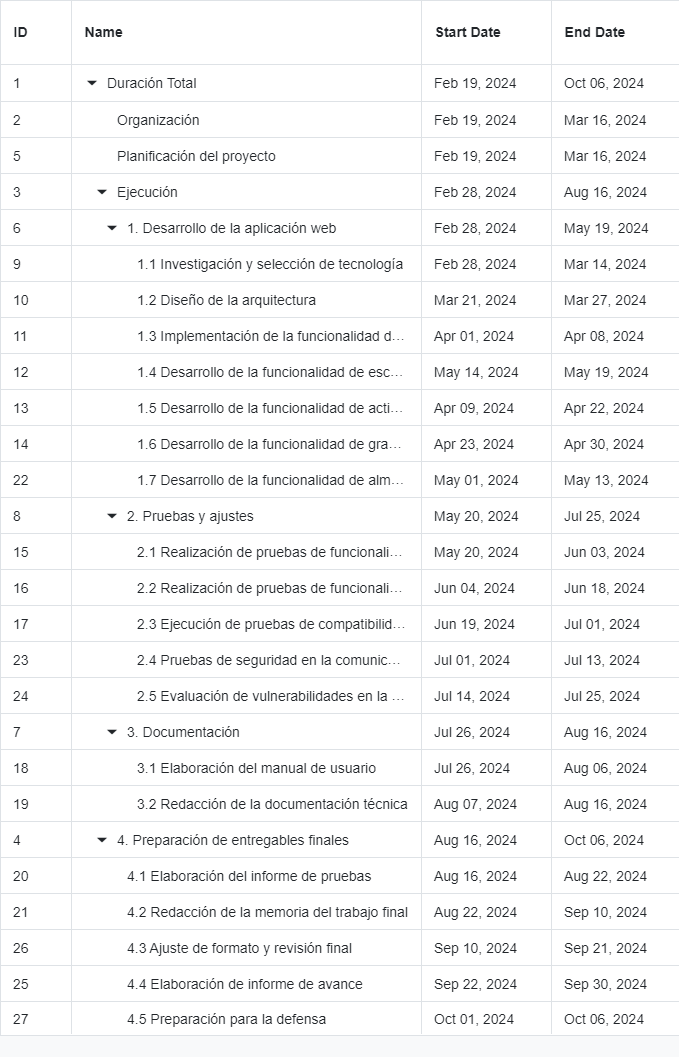
\includegraphics[width=.73\textwidth]{./Figuras/tasks.png}
\caption{Tareas del plan de proyecto.}
\label{fig:Tasks}
\end{figure}

\begin{figure}[htpb]
    \centering 
    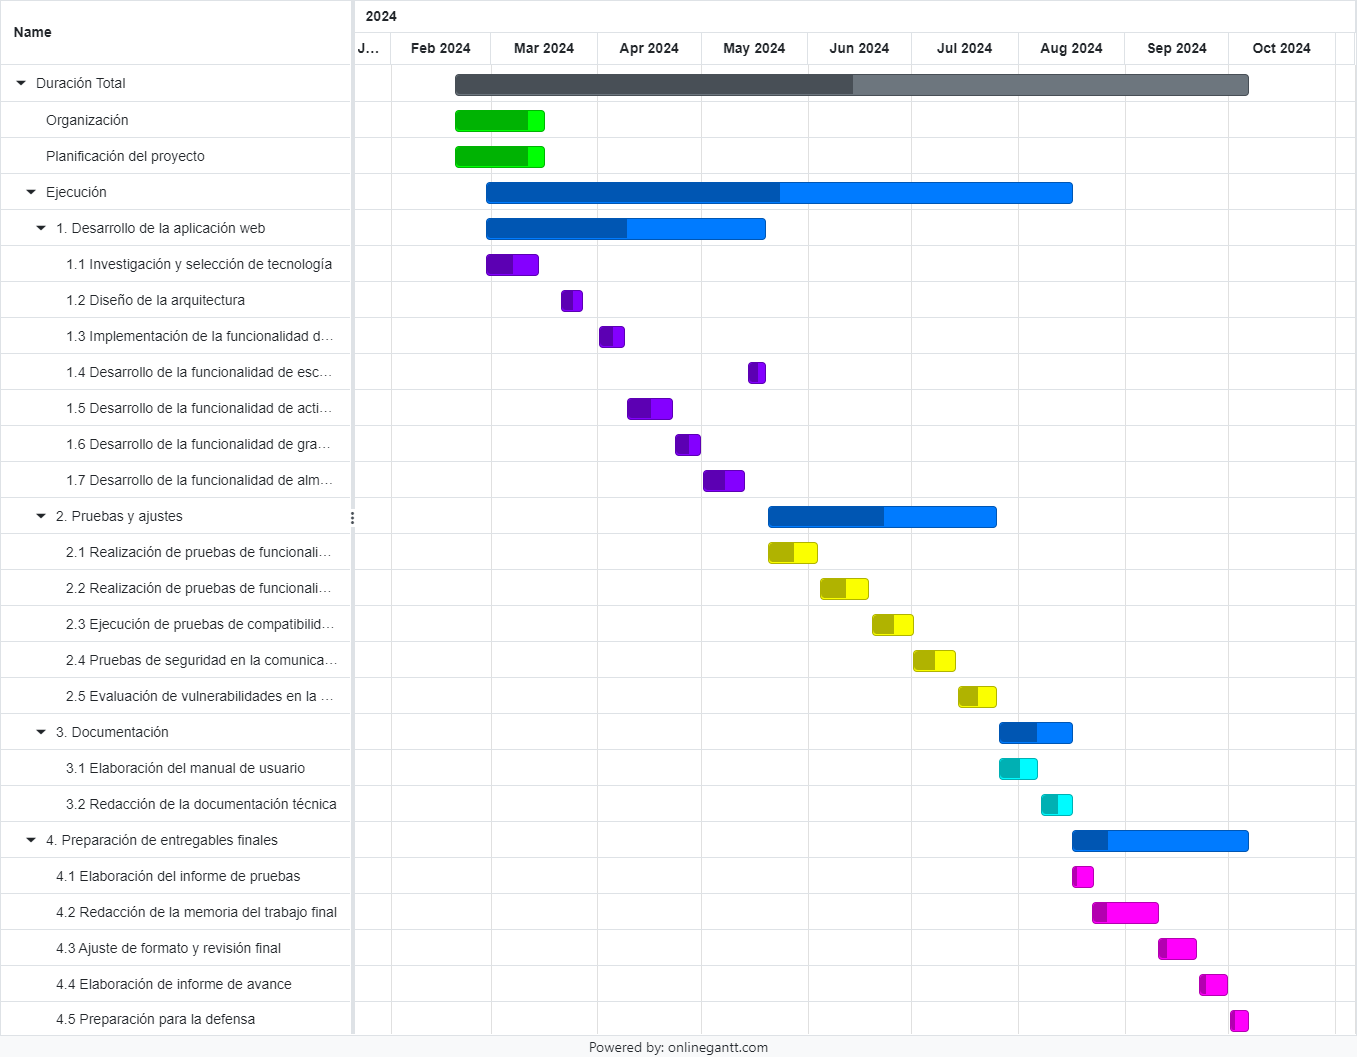
\includegraphics[width=1\textwidth]{./Figuras/gantt_.png}
    \caption{Diagrama Gantt del presente proyecto.}
    \label{fig:Gantt}
\end{figure}


\section{12. Presupuesto detallado del proyecto}
\label{sec:presupuesto}

El presupuesto del presente proyecto inicialmente fue calculado en dólares americanos. Sin embargo, bajo una tasa de cambio 1 USD = 856.74 ARS a la fecha del 26 de marzo de 2024, los valores equivalentes en la divisa argentina se muestran en la siguiente tabla.
\begin{table}[htpb]
\centering
\begin{tabularx}{\linewidth}{@{}|X|c|r|r|@{}}
\hline
\multicolumn{4}{|c|}{\cellcolor[HTML]{C0C0C0}COSTOS DIRECTOS} \\ \hline
\rowcolor[HTML]{C0C0C0} 
Descripción &
  \multicolumn{1}{c|}{\cellcolor[HTML]{C0C0C0}Cantidad} &
  \multicolumn{1}{c|}{\cellcolor[HTML]{C0C0C0}Valor unitario} &
  \multicolumn{1}{c|}{\cellcolor[HTML]{C0C0C0}Valor total} \\ \hline
 Horas de ingeniería. &
  \multicolumn{1}{c|}{580} &
  \multicolumn{1}{c|}{\$ 8138,97} &
  \multicolumn{1}{c|}{\$ 4232266,95} \\ \hline
 Componentes varios. &
  \multicolumn{1}{c|}{1} &
  \multicolumn{1}{c|}{\$ 1206.87} &
  \multicolumn{1}{c|}{\$ 1206.87} \\ \hline
\multicolumn{3}{|c|}{SUBTOTAL} &
  \multicolumn{1}{c|}{\$ 4352953,95} \\ \hline
\rowcolor[HTML]{C0C0C0} 
\multicolumn{4}{|c|}{\cellcolor[HTML]{C0C0C0}COSTOS INDIRECTOS} \\ \hline
\rowcolor[HTML]{C0C0C0} 
Descripción &
  \multicolumn{1}{c|}{\cellcolor[HTML]{C0C0C0}Cantidad} &
  \multicolumn{1}{c|}{\cellcolor[HTML]{C0C0C0}Valor unitario} &
  \multicolumn{1}{c|}{\cellcolor[HTML]{C0C0C0}Valor total} \\ \hline
Mes de alojamiento web. &
  \multicolumn{1}{c|}{6} &
  \multicolumn{1}{c|}{\$ 12851,13} &
  \multicolumn{1}{c|}{\$ 77106,78} \\ \hline
\multicolumn{3}{|c|}{SUBTOTAL} &
  \multicolumn{1}{c|}{\$ 77106,78} \\ \hline
\rowcolor[HTML]{C0C0C0}
\multicolumn{3}{|c|}{TOTAL} & \$ 4430060,73
   \\ \hline
\end{tabularx}%
\end{table}


\section{13. Gestión de riesgos}
\label{sec:riesgos}
Durante el desarrollo del plan de proyecto, se han detectado los riesgos potenciales detallados a continuación. De igual manera, se establece un plan de mitigación para aquellos que superen un criterio determinado especificado posteriormente.

Para la ponderación de severidad y ocurrencia de cada uno de los riesgos se hará uso de una escala de valores enteros entre 1 y 10.

\begin{itemize}
    \item Riesgo 1: pérdida de conexión al servidor.
    \begin{itemize}
        \item Severidad (S): 8
        \item Probabilidad de ocurrencia (O): 6
        \item Descripción: la pérdida de conexión al servidor podría ocurrir debido a fallas en la red o problemas de infraestructura, lo que afectaría la disponibilidad y funcionalidad del sistema.
    \end{itemize}
    
    \item Riesgo 2: vulnerabilidad en la habilitación de cerradura por BLE (Bluetooth Low Energy).
    \begin{itemize}
        \item Severidad (S): 9
        \item Probabilidad de ocurrencia (O): 5
        \item Descripción: la presencia de vulnerabilidades en la habilitación por BLE podría exponer el sistema a ataques de seguridad, comprometiendo la integridad y confidencialidad de los huéspedes.
    \end{itemize}
    
    \item Riesgo 3: imposibilidad de probar el código en hardware.
    \begin{itemize}
        \item Severidad (S): 7
        \item Probabilidad de ocurrencia (O): 4
        \item Descripción: la falta de acceso o la imposibilidad de probar el código en hardware real podría dificultar la validación y optimización del sistema, aumentando el riesgo de errores en la implementación final.
    \end{itemize}
    
    \item Riesgo 4: falta de actualización o mantenimiento de las tecnologías utilizadas.
    \begin{itemize}
        \item Severidad (S): 7
        \item Probabilidad de ocurrencia (O): 3
        \item Descripción: si las tecnologías utilizadas en el proyecto no se actualizan o mantienen adecuadamente, podría surgir la incompatibilidad con versiones futuras de sistemas operativos o dispositivos, lo que podría afectar la funcionalidad y la seguridad del sistema.
    \end{itemize}
    
    \item Riesgo 5: interrupción del suministro de energía o fallo de hardware.
    \begin{itemize}
        \item Severidad (S): 8
        \item Probabilidad de ocurrencia (O): 4
        \item Descripción: un fallo en el suministro de energía o un fallo del hardware en el servidor o los dispositivos móviles podría causar una interrupción en el funcionamiento del sistema, lo que afectaría la seguridad y la experiencia del usuario.
    \end{itemize}
\end{itemize}

b) Tabla de gestión de riesgos: (El RPN se calcula como RPN=SxO)
\begin{table}[htpb]
\centering
\begin{tabularx}{\linewidth}{@{}|X|c|c|c|c|c|c|@{}}
\hline
\rowcolor[HTML]{C0C0C0} 
Riesgo & S & O & RPN & S* & O* & RPN* \\ \hline
Pérdida de conexión al servidor & 8 & 6 & 48 & 6 & 5 & 30 \\ \hline
Vulnerabilidad en la habilitación por Bluetooth & 9 & 4 & 36 & 7 & 4 & 28 \\ \hline
Imposibilidad de probar el código en hardware & 7 & 5 & 35 & 6 & 3 & 18 \\ \hline
Falta de actualización o mantenimiento de las tecnologías utilizadas & 7 & 3 & 21 & - & - & - \\ \hline
Interrupción del suministro de energía o fallo de hardware & 8 & 4 & 32 & - & - & - \\ \hline
\end{tabularx}%
\end{table}

c) Plan de mitigación de riesgos:

Para los riesgos con un RPN mayor o igual a 35, se implementarán las siguientes medidas de mitigación:

Riesgo 1: se implementarán medidas de redundancia y monitoreo para minimizar el impacto de la pérdida de conexión al servidor.
\begin{itemize}
    \item Severidad (S): se reduce a 6. Esto se debe a que la implementación de medidas de redundancia y monitoreo reduce el impacto negativo de la pérdida de conexión al servidor, lo que disminuye la gravedad de las consecuencias en caso de que ocurra.
    \item Probabilidad de ocurrencia (O): se reduce a 5. La ocurrencia de este evento no depende del sistema en sí, mas de incidentes respecto al servidor y su arquitectura. Sin embargo, las estrategias de reconexión rápida son una repuesta oportuna ante el riesgo.
\end{itemize}


Riesgo 2: se realizarán pruebas exhaustivas de seguridad durante el desarrollo para identificar y corregir cualquier brecha de seguridad potencial.
\begin{itemize}
\item Severidad (S): se reduce a 7. La implementación de medidas de seguridad adicionales reduce la gravedad de las posibles consecuencias en caso de una vulnerabilidad en la habilitación por BLE.
\item Probabilidad de ocurrencia (O): se reduce a 4. La adopción de buenas prácticas de seguridad ante posibles amenazas disminuyen la probabilidad de que ocurra una vulnerabilidad en la habilitación por BLE.
\end{itemize}

Riesgo 3: se establece una colaboración estrecha con SURiX para contar con opciones de simulación del entorno de hardware o, a su vez, la ejecución del sistema a nivel local para correr pruebas exhaustivas del código.
\begin{itemize}
\item Severidad (S): se reduce a 6. La implementación de escenarias de simulación, junto con la colaboración de SURiX, reduce la gravedad de la imposibilidad de probar el código en hardware real, permitiendo una validación parcial del sistema.
\item Probabilidad de ocurrencia (O): se reduce a 3. Establecer acuerdos de colaboración con una empresa de tal trayectoria disminuye la probabilidad de que ocurra la imposibilidad de probar el código en hardware real.
\end{itemize}

\section{14. Gestión de la calidad}
\label{sec:calidad}
\begin{itemize}
\item Req \#6.1.1: los usuarios deben poder visualizar la información de la propiedad correspondiente para alquiler temporal.
\begin{itemize}
\item Verificación: realizar pruebas con diferentes usuarios y dispositivos para asegurar la usabilidad.
\item Validación: analizar la interfaz de usuario durante la visualización de información de diferentes propiedades.
\end{itemize}

\item Req \#6.1.2: los usuarios deben poder utilizar los periféricos de su teléfono móvil para interactuar con la aplicación.
    \begin{itemize}
        \item Verificación: simular la interacción con diferentes periféricos en la aplicación y revisar el código fuente para confirmar la integración adecuada.
        \item Validación: observar la experiencia del usuario durante la interacción con los periféricos durante el período de pruebas con SURiX.
    \end{itemize}

    \item Req \#6.1.3: la aplicación web debe proporcionar una funcionalidad de escaneo de códigos QR para acceder a la información de la propiedad.
    \begin{itemize}
        \item Verificación: implementar y probar el escaneo de códigos QR, y verificar la correcta visualización de la información.
        \item Validación: evaluar la facilidad de uso y precisión del escaneo, realizando pruebas en diferentes condiciones de iluminación.
    \end{itemize}

    \item Req \#6.1.4: una vez escaneado el código QR, la aplicación debe proporcionar al usuario la información necesaria para conectarse por Bluetooth con la cerradura electrónica de la propiedad.
    \begin{itemize}
        \item Verificación: desarrollar y probar la funcionalidad de conexión Bluetooth, y verificar la correcta visualización de la información de conexión.
        \item Validación: solicitar a SURiX pruebas de conexión Bluetooth con su cerradura electrónica y evaluar la confiabilidad y seguridad de la conexión.
    \end{itemize}

    \item Req \#6.1.5: la aplicación debe permitir al usuario abrir o cerrar la cerradura electrónica utilizando la funcionalidad de activación Bluetooth.
    \begin{itemize}
        \item Verificación: implementar y probar la función de apertura/cierre de la cerradura, y verificar la respuesta adecuada de la cerradura a las órdenes de la aplicación.
        \item Validación: solicitar a SURiX pruebas de apertura/cierre en diferentes escenarios y evaluar la seguridad y confiabilidad de la función.
    \end{itemize}

    \item Req \#6.1.6: el sistema debe notificar al propietario cuando la cerradura electrónica se abre o se cierra.
    \begin{itemize}
        \item Verificación: implementar y probar la funcionalidad de notificaciones, y verificar el envío correcto de las mismas.
        \item Validación: solicitar al cliente pruebas de recepción de notificaciones en diferentes situaciones y evaluar la puntualidad y precisión de las mismas.
    \end{itemize}

    \item Req \#6.1.7: la aplicación web debe facilitar la comunicación entre el inquilino y el propietario mediante mensajes de voz.
    \begin{itemize}
        \item Verificación: implementar y probar la funcionalidad de envío y recepción de mensajes de voz, y verificar la calidad adecuada del audio.
        \item Validación: junto con SURiX realizar pruebas de la funcionalidad en diferentes condiciones de audio y evaluar la efectividad de la comunicación.
    \end{itemize}

    \item Req \#6.4.1:la interfaz de usuario debe ser intuitiva y fácil de navegar.
   \begin{itemize}
            \item Verificación: realizar pruebas de usabilidad con diferentes usuarios, observar la facilidad de navegación y solicitar feedback sobre la facilidad de uso de la interfaz.
            \item Validación: analizar los resultados de las pruebas de usabilidad, implementar mejoras en la interfaz basadas en el feedback de los usuarios y realizar pruebas adicionales para confirmar la efectividad de las mejoras.
        \end{itemize}

    \item Req \#6.4.2: se debe proporcionar retroalimentación visual para confirmar las acciones realizadas por el usuario, como el acceso a la propiedad o el envío de un mensaje de voz.
        \begin{itemize}
            \item Verificación: implementar la funcionalidad de retroalimentación visual en la aplicación, probarla con diferentes acciones y verificar su claridad y comprensibilidad.
            \item Validación: solicitar al cliente que pruebe la retroalimentación visual en diferentes escenarios y evaluar su utilidad y eficacia.
        \end{itemize}

    \item Req \#6.4.3: la aplicación debe contar con un diseño \textit{responsive} que se adapte automáticamente a diferentes tamaños de pantalla.
        \begin{itemize}
            \item Verificación: implementar un diseño responsive, probar la aplicación en diferentes dispositivos con diferentes tamaños de pantalla y verificar su correcta adaptación.
            \item Validación: solicitar al cliente que pruebe la aplicación en diferentes dispositivos y evaluar la calidad del diseño responsive y la experiencia del usuario en cada uno.
        \end{itemize}
    \end{itemize}


\section{15. Procesos de cierre}    
\label{sec:cierre}

\begin{itemize}
    \item Pautas de trabajo que se seguirán para analizar si se respetó el plan de proyecto original:\newline
       - Reuniones mensuales con el cliente para la verificación del cumplimiento de tareas.
       - Retroalimentación quincenal con el orientador del proyecto para control de avance y solución de inconvenientes.

    \item Identificación de las técnicas y procedimientos útiles e inútiles que se emplearon, los problemas que surgieron y cómo se solucionaron:\newline
       - Evaluación por parte del equipo de proyecto de las técnicas y procedimientos utilizados, así como de los problemas surgidos y sus soluciones aplicadas.

    \item Organización del acto de agradecimiento a todos los interesados, y en especial al equipo de trabajo y colaboradores:\newline
       - La responsable del proyecto organizará el acto de agradecimiento y reconocimiento a todos los interesados, incluyendo al equipo de trabajo y colaboradores. Los gastos correspondientes serán financiados por el presupuesto del proyecto.
\end{itemize}

\end{document}